\chapter{Introduction}

\section{\texorpdfstring{Link Prediction \normalfont{\emoji{mag}}}{Link
      Prediction}} \label{link-prediction-mag}

\textbf{\emph{Definition \normalfont{\emoji{key}}:}} Link prediction finds missing links
(in static networks) or predicts the likelihood of future links (in
dynamic networks).\\

There exists a wide range of link prediction techniques like
similarity-based indices, probabilistic methods, dimensionality
reduction approaches, etc.

\section{Background}

A \textbf{social network} (a more general term is a complex network) is a
standard approach to model communication in a group or community of persons.
Such networks can be represented as a graphical model in which a node maps to a
person or social entity, and a link corresponds to an association or
collaboration between corresponding persons or social entities. When links can
be deleted or added, during time, the network is called \textbf{dynamic}. Lots
of issues arise when we study a social network, some of which are changing
association patterns over time, factors that drive those associations, and the
effects of those associations to other nodes. Here, we address a specific
problem termed as link prediction.

\paragraph{Problem Characterization.}\label{problem-characterization}
Consider a simple undirected network \(G(V, E)\) (Refer to the Figure 1), where
\(V\) characterizes a vertex-set and \(E\), the link-set.

\begin{figure}[H]
    \centering
    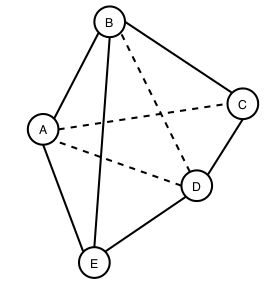
\includegraphics[width=4cm, keepaspectratio]{capitoli/intro/imgs/img1.png}
    \caption{Network representation as a graph}
\end{figure}

We use (\texttt{vertex $\equiv$ node}), (\texttt{link $\equiv$ edge}) and
(\texttt{graph $\equiv$ network}) interchangeably. In the graph, a universal set
\(U\) contains a total of \(\frac{n(n-1)}{2}\) links (total node-pairs), where
\(n = |V|\) represents the number of total vertices of the graph. (\textbar
U\textbar{} - \textbar E\textbar) number of links are termed as the
\emph{non-existing links}, and some of these links may appear in the near future
when we talk about dynamic network. \textbf{\emph{Finding such missing links
        (i.e., AC, BD, and AD) is the aim of link prediction}}.\\

The link prediction problem can be defined as follow: \emph{Suppose a graph
    $G_{t_0 - t_1} (V, E)$ represents a snapshot of a network
    during time interval $[t_0 ,t_1]$ and $E_{t_0 -
                t_1}$, a set of links present in that snapshot. The task of link
    prediction is to find set of links $E_{t_0' - t_1'}$ during
    the time interval $[t_0' ,t_1']$ where $[t_0 ,t_1]
        \leq [t_0' ,t_1']$.}\\

The link prediction idea is useful in several domains of application. Examples
include automatic hyperlink creation, website hyper-link prediction in the
Internet and web science domain, and friend recommendation on Facebook.